\documentclass{article} % For LaTeX2e
\usepackage{nips12submit_e,times}
\usepackage{amsmath}
\usepackage{graphicx}
%\usepackage{caption}
\usepackage{subcaption}
\usepackage{comment}
\usepackage{hyperref}
\usepackage{url}
\usepackage[top=1.0in, bottom=1.0in, left=1.0in, right=1.0in]{geometry}

%\renewcommand\refname{Papers To Read}
\title{Semantic Segmentation Using Label Propagation}

\author{
Aravindh Mahendran \\
\texttt{amahend1@andrew.cmu.edu} \\ 
\And
Nitish Thatte \\
\texttt{nitisht@andrew.cmu.edu} \\
\AND
Adwait Gandhe \\
\texttt{agandhe@andrew.cmu.edu} \\
}

\newcommand{\fix}{\marginpar{FIX}}
\newcommand{\new}{\marginpar{NEW}}

\nipsfinalcopy

\begin{document}
\maketitle

\begin{abstract}
Semantic image segmentation is the process of assigning human relevant labels to pixels in an image and is a high level vision problem. Increasing the number of labels increases the complexity of the problem. In this work we attempt a supervised learning approach to solve this problem by training a classifier that helps propagate labels to improve upon a generative prior. We present our results on the 13 class MSRC V1 Dataset.
\end{abstract}


\section{Introduction}
Semantic segmentation is the process of assigning a class label to each pixel of the image. This is an important problem in computer vision for understanding the underlying information in an image. While classical segmentation techniques group together the pixels based on low level features, semantic segmentation adopts a supervised learning approach. There are two common approaches for semantic segmentation. The first makes use of low level features and combines them with a learning framework to obtain higher level labels. The second approach is to use low level cues, rather than features, with random fields and learn a unified framework using low level segmentation. In this paper, we first estimate the probability for every pixel label pair by using the k-Nearest Neighbors and the Bag of Words model. A Random Forest \cite{Statistics01randomforests} using the color and texton features is trained which decides whether two connected super pixels share a label and the direction in which the label is propagated. 

This paper is structured as follows: Section \ref{sec:Problem} discusses the problem statement. Section \ref{sec:Related} talks about the related work. Section \ref{sec:Proposed} discusses our method for semantic image segmentation. The experiments conducted and the results obtained are presented in section \ref{sec:Exp}. Finally we summarize our conclusions in section \ref{sec:Conclusion}.
\label{sec:Intro}

\subsection{Related Work}
\label{sec:Related}
One of the first approaches for simultaneous object segmentation and recognition utilizes an Implicit Shape Model that integrates both capabilities into a common probabilistic framework \cite{Leibe04combinedobject}. 
Another approach used a generative model based on the bag of words representation for such simultaneous recognition and segmentation \cite{cao:spatially}.  
Furthermore, a method based on some of these approaches for scoring low-level patches according to their class relevance and propagating these posterior probabilities to pixels has been developed \cite{conf/bmvc/CsurkaP08}.

Several recent approaches use random fields to incorporate local cues and impart global control without implementing low level segmentation. For example, \cite{Kumar:2005:OC:1068507.1068889} proposes a Bayesian method for combining top-down and bottom-up cues. Conditional random fields have also been used for this purpose \cite{Kumar:2005:HFF:1097115.1097790} \cite{Richard04multiscaleconditional}. Finally, Textonboost \cite{Shotton06textonboost:joint} is an approach to learning a discriminative model of object classes incorporating appearance, shape and context information efficiently. We suggest \cite{SegmentRegionsParts} for other semantic image segmentation approaches.
%------------------------------------------------------------------------------------------

\subsection{Problem Definition}
\label{sec:Problem}

%------------------------------------------------------------------------------------------
\section{Proposed Method}
\label{sec:Proposed}
\subsection{Intuition}
\subsection{Our Approach}
\subsubsection{Features}
\paragraph{Textons}
Textons represent texture information.
A collection of filters is used to process each pixel to obtain a per
pixel feature vector.
This is quantized to a single number by selecting a vector nearest to the
current one from a precomputed dictionary.
If each vector in the dictionary is considered to be a word, this
representation gives one word per image pixel and is called the TextonMap
or WordMap. %TODO: Insert figure
A bag of words histogram is computed for each super pixel or segment by
counting word occurrences.
We used the filter bank and dictionary provided by \cite{malisiewicz-cvpr08}.

\paragraph{Color}
Color information is important for separating classes that lack texture or
have similar texture.
We use the per channel color histogram, color mean and standard deviation
from the HSV color space.
\subsubsection{Label Propagation}
\label{sec:labprop}
\paragraph{Super pixels and connectivity graph}
Each image is divided into super pixels at two different scales such that
the a coarse super pixels align with corresponding finer ones.
This is achieved by using \cite{}.%TODO Cite the super pixel people.
A graph is constructed where each fine super pixel is connected to its
4-connected neighborhood and to all fine super pixels inside the same
coarse super pixel.
We believe that this connectivity helps model non local properties which
are important for determining semantically relevant class labels.

\paragraph{Training the classifier}
We train a classifier that decides whether or not two super pixels should
have the same label.
We assign a label for each super pixel by taking the majority vote over
ground truth labels of each pixel in it.
Each edge in the super pixel graph of a training image is considered a
positive sample if corresponding super pixels have the same label,
negative other wise.
This training data is collected over the k nearest neighbors to the test
image and used to train a random forest.
If done this way, we have too many positive samples and too few negatives
and discriminative learning fails to separate them.
We resample the training data to ensure a low enough ratio between these
before training our classifier.
Note that we train a new random forest for every test image.
Texton and color features are concatenated to describe each super pixel.
Further, each edge in the graph is described by the absolute difference of
their features.

\paragraph{Propagating Labels}
A different segmentation algorithm (see section \ref{baseline}) gives a
probability for each pixel label pair.
The entropy for each super pixel can be calculated from this distribution.
The label with highest probability is treated as the label assigned to
each pixel.
A majority vote over this assignment is used to determine the label for
each super pixel.
When the baseline is inconsistent with the prediction of our random
forest, we propagate labels from the super pixel with higher entropy to
the super pixel with lower entropy.
This propagation is run from the lowest entropy super pixel to the highest
entropy super pixel propagating labels to super pixels further down in
this sorted list.

\subsubsection{Baseline}
\label{baseline}
The label propagation approach discussed above requires per pixel values
for $P(Label)$.
The algorithm which provides this is referred to as baseline and described
below in detail.

\paragraph{Training} Each training image is divided into segments using
Meanshift based EDISON \cite{meanshift}.
A normalized texton histogram (bag of words representation) is computed for each segment.
The ground truth label for each segment is selected by taking a majority vote over per pixel ground truth labels.

\paragraph{Testing} For each test image, meanshift segments and normalized texton histograms of the same are computed.
A new model is trained from the GIST feature based nearest neighbors for the given test image.
The probability distribution $P(Label | feature)$ is computed by counting the occurrences of each label in the K nearest segments from the training data.
This distribution is copied to each pixel in the image and a per pixel distribution and entropy is thus available.

\subsection{Other Attempted Methods}
\subsubsection{HMLN}
Markov Logic Networks \cite{Domingos06unifyinglogical} \cite{Richardson06markovlogic} attach weights to first-order formulae and view them as templates for building Markov Networks. Hybrid Markov Logic Networks (HMLNs)\cite{Wang_hybridmarkov} are an extension that allow for continuous properties to appear as features. Hybrid Markov Logic Networks combine logic and probabilistic inference techniques. This provides a powerful tool for solving high level problems such as semantic segmentation which involve complexity and noise. Our initial approach till the mid term report was based on an implementation of this tool called Alchemy \cite{alchemy}. This attempt, however, failed due to bugs in the implementation and memory issues causing lack of scalability to our dataset. 

\subsubsection{SVM for Label Propagation}
We experimented with SVM's in place of random forests and found them to not converge when training on the entire dataset. Training on the nearest neighbors of a test image lead to convergence but the results were too bad to be used.

\subsubsection{Conditional Random Fields}
Conditional random fields \cite{lafferty2001conditional} are undirected graphical models that can perform inference to compute marginal distributions of label probabilities given features.
We attempted to use these for generating baseline segmentations using the Ising model with each pixel as a node.
These, however, are computationally expensive as they have loops.
We experimented with pseudo log likelihood training and loopy belief propogation using the UGM toolbox\cite{UGMSoftware}.
The maximum aposteriori estimate of label assignments to image pixels always labeled each pixel as Grass.
This was due to a very high unary potential learnt for the corresponding node. 
We did not pursue this approach due to very high computational requirements.
Furthermore, loopy belief propogation did not converge after more than 6 hours of training.

\subsection{Adaboost}
We explored used Adaboost instead of random forests but random forests gave better results on the classification task.

%------------------------------------------------------------------------------------------


%------------------------------------------------------------------------------------------
\section{Experiments}
\label{sec:Exp}


\subsection{Description of Experiments}
\label{sec:Description}

\subsubsection{Cross Validation}
\label{sec:cross}
We tested our algorithm on the MSRC V1 Dataset \cite{MSRC}, which we randomly into 100 test images 20 validation images and 100 training images.
Superpixels and connectivity graphs for all the images were precomputed and stored.
Then, we performed leave-one-out cross validation to optimize the parameters in the algorithm.
These parameters are $k_{bag}$ for the $k$-nearest-neighbor images from which the bag of words model is computed, $k_{hist}$ for the $k$-nearest-neighbor Texton histograms from which the distribution $P(Label | feature)$ is generated, $k_{forest}$ for the $k$-nearest-neighbors used by the random forest, and a ratio parameter used to balanced the number true and false edges on the connectivity graph. 

Due to a lack of computational resources, optimizing these four parameters simultaneously proved intractable. Therefore, the we assumed that the parameters for the bag-of-words model and the random forest affect the final segmentation independently. This assumption is supported by the relative magnitudes by which the parameters affect the accuracy of the semantic segmentation

\begin{figure}[htb]
\centering
	\begin{subfigure}[t]{0.33\textwidth}
		\centering
		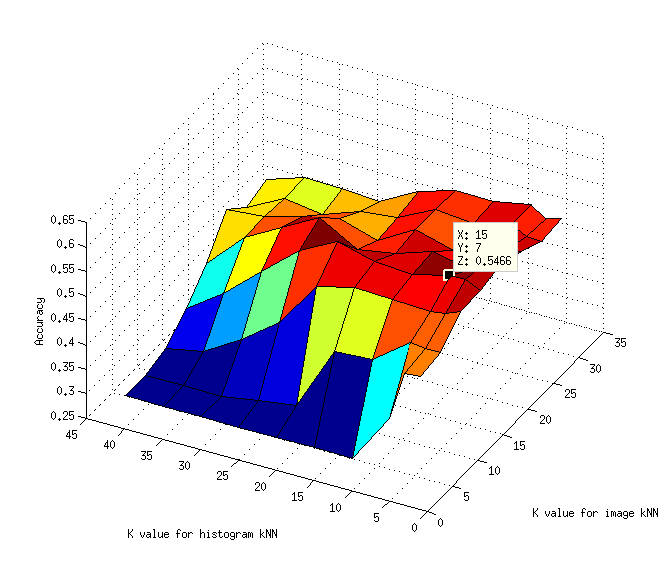
\includegraphics[width = \textwidth]{./img/pickK_final}
		\parbox{.95\textwidth}{\caption{Accuracy versus bag of words model parameters obtained from leave-one-out cross validation. The chosen parameters $k_{imgs} = 15$, and $k_{histo} = 7$ are highlighted. \label{fig:Kbag} }}
			\end{subfigure}
	\begin{subfigure}[t]{0.33\textwidth}
		\centering
		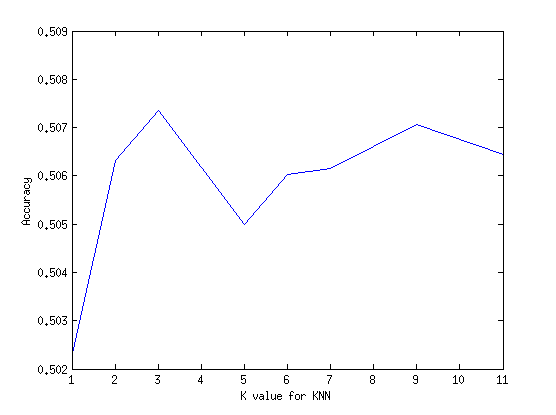
\includegraphics[width = \textwidth]{./img/kforest}
		\parbox{0.95\textwidth}{\caption{Accuracy versus $k_{forest}$ obtained from leave-one-out cross validation. $k_{forest} = 9$ was chosen. \label{fig:Kforest}}}
	\end{subfigure}
	\begin{subfigure}[t]{0.33\textwidth}
		\centering
		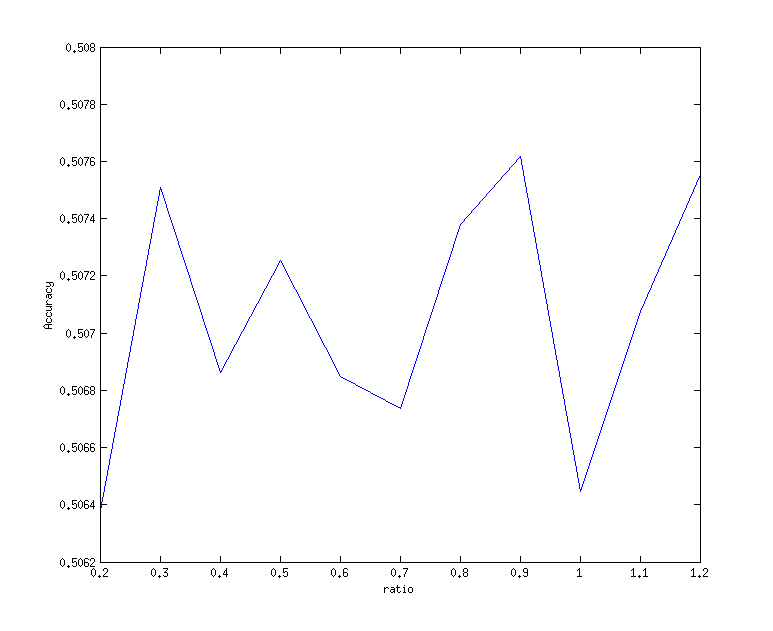
\includegraphics[width = \textwidth]{./img/ratio}
		\parbox{0.95\textwidth}{\caption{Accuracy versus true/false points ratio obtained from leave-one-out cross validation. A ratio  of 0.5 was chosen. \label{fig:ratio}}}
	\end{subfigure}
\end{figure}

Figure \ref{fig:Kbag} shows the accuracy of the final segmentations of the validation images with respect to the bag of words model parameters. For this test, the parameters for the random forest, $k_{forest}$ value and ratio, were set 11 and 0.8 respectively. We chose a set of parameters that produced a high accuracy result and also had low first and second derivatives. We believe low derivatives are desirable as they indicate stability and therefore characterize parameters that generalize well to the test data. Consequently, we chose $k_{bag} = 15$, and $k_{hist} = 7$ as these parameters satisfy these properties.

The next parameter we validated was the number of nearest neighbor images on which to train the random forest, $k_{forest}$. Figure \ref{fig:Kforest} shows the result of the leave-one-out cross validation on this parameter. This plot shows that for accuracy is roughly constant for all $k_{forest}$ except for a value of 1, for which it is markedly decreased. While this plot shows no conclusive reason to choose one $k$ value over another, high $k$ values result in more data points and thus should decrease the variability of the results. However, larger values of $k_{forest}$ such as 11 or 13, resulted in unacceptably slow training times. Therefore, we chose $k_{forest} = 9$ as it represented an acceptable compromise between these features.

The last varied parameter was the ratio of sampled true points to false points used in the training data for the random forest. This parameter is vital, as the graph structure proposed in section \ref{sec:labprop} results in a far greater number of same-labeled superpixel pairs than differently-labeled superpixel pairs. Without this parameter, all tested classifiers tended to fit to the positive labeled points almost exclusively, resulting in high precision and recall but near-zero specificity. For our application, this is extremely undesirable, as a false-positive, resulting in the classifier propagating a label when it should not have, can only degrade the segmentation. For high ratio values, (0.8 - 1.2) this same behavior was observed, as suggested in the variability of the plot in this range. We chose a ratio of 0.5 for our final classifier, as it resulted in very high specificity values, and ensured that the label propogation indicator would be conservative. 


\subsection{Observations}

\label{sec:Observations}

%------------------------------------------------------------------------------------------

\section{Conclusion}
\label{sec:Conclusion}

\bibliographystyle{plain}
\bibliography{final_report}

\end{document}
